\documentclass[a4paper,12pt]{article}
\usepackage[utf8]{inputenc}
\usepackage[brazilian]{babel}

\usepackage{mathptmx}               %Times New Roman
\usepackage{newtxtext,newtxmath} 

\usepackage{setspace}
\setstretch{1}      % Espacio entre lineas

\usepackage{vmargin}
\setpapersize{A4}
\setmargins{3cm}	% margen izquierdo
{1.5cm}            	% margen superior
{15cm}          	% anchura del texto
{23.5cm}          	% altura del texto
{10pt}             	% altura de los encabezados
{1cm}              	% espacio entre el texto y los encabezados
{0pt}              	% altura del pie de página
{1.5cm}             % espacio entre el texto y el pie de página

\usepackage{cite}

\usepackage{flushend}
\usepackage{amsmath}
\usepackage{textcomp}

\usepackage{multirow}

\usepackage[usenames]{color}
\usepackage[hidelinks]{hyperref} 

\usepackage{enumitem,kantlipsum}

\usepackage{graphicx} % figuras
\usepackage[export]{adjustbox}
\usepackage[labelfont=bf]{caption} %Negrita al label de la figura
\usepackage[font=it]{caption} %Italica descripcion de la figura 

\usepackage{fancyhdr,lipsum} %Encabezados
\pagestyle{fancy}
\setlength{\headheight}{52pt}

\fancypagestyle{plain}{
\fancyhead[L]{}
\fancyhead[R]{CAP-241-4 - Computação Aplicada}
\setlength{\headheight}{15pt}
\renewcommand{\headrulewidth}{0.5pt}}

\usepackage{subcaption}

\usepackage{breqn}

\begin{document}
\begin{figure}
 \begin{center}
  
\includegraphics[width=1\linewidth]{fig/logoinpe.png}
 \end{center}
\end{figure}

\setlength{\textfloatsep}{0pt}

\title{Modelando Epidemias Usando Autômatos Celulares}
    
\author{Arturo Sánchez Pena \\ Felipe Menino Carlos}
\date{}

\maketitle

\section{Introdução}

Modelos são formas de representação simplificadas de sistemas da natureza e seus comportamentos, utilizados para que os pontos mais importantes e relevantes sejam vistos e compreendidos (KIER 2005\cite{Kier2005}). Diversos estudos usam de modelos para o entendimento do comportamento geral de sistemas da natureza com os mais diferentes objetivos e necessidades. Alguns exemplos podem ser encontrados em, Cairo 2019 \cite{Cairo2019}, que utiliza de modelos estatísticos para a modelagem de concentração de chl-\textit{a} através de dados de Sensoriamento Remoto. Outro exemplo está em ZORZENON \textit{et al} \cite{ZorzenonDosSantos2001}, que através de modelagem estuda a evolução do Vírus da Imunodeficiência Humana (HIV). Estes e diversos outros exemplos deixam claro a importância da utilização de modelos e os avanços que o processo de modelagem traz para os mais variados contextos.

O processo de modelagem pode ser feito através da utilização de diversas técnicas (KIER 2005\cite{Kier2005}). Atualmente, dentre as técnicas utilizadas está o Autômato Celular (AC), que através de um conjunto de regras simples, permitem a modelagem de sistemas e comportamentos complexos (MELOTTI 2009\cite{Melotti2009}).

Por conta de seu grande por de expressão de problemas, a modelagem baseada em ACs vem sendo amplamente explorada em trabalhos relacionados ao comportamento de doenças e suas dinâmicas de disseminação. Tal abordagem tem ganhado notoriedade por seus bons resultados e por permitir que os mais variados contextos de epidemias sejam facilmente modelados, o que em situações reais pode ser extremamente útil para a tomada de decisões por parte de instituições públicas e privadas na contenção de possíveis epidemias.

Desta forma, o presente trabalho tem por objetivo implementar e analisar os resultados do modelo de AC proposto por White 2007 \cite{White2007}, que busca ser uma alternativa geral para a modelagem de diferentes tipos de epidemias. 

\section{Autômatos celulares}
\par ACs são modelos matemáticos que tornam possível a representam de sistemas e fenômenos dinâmicos (MELOTTI 2009 \cite{Melotti2009} e CASTRO 2008 \cite{Castro2008}), tornando esses ferramentas úteis para a modelagem de diferentes tipos de comportamento, sendo empregados nos mais variados contextos (CASTRO 2008\cite{Castro2008}). Por sua capacidade de expressar comportamentos dinâmicos, os ACs são frequentemente descritos como contrapartes às equações diferenciais (MELOTTI 2009\cite{Melotti2009}), sendo utilizados em muitos trabalhos por conta de sua fácil representação e grande poder de expressão de diferentes comportamentos. Melotti 2009\cite{Melotti2009} afirma que, a ideia por trás da utilização de ACs para a descrição de sistemas e fenômenos é buscar fazer a representação desses não por meio de equações complexas, mas sim, simular tais sistemas e permitir que a interação do mesmo entre seus componentes, por meio de regras simples, gere os mesmos comportamentos que estão sendo modelados. 

\subsection{Componentes de um autômato celular}
Liu 2008 \cite{Liu2008} especifica que os autômatos celulares possuem cinco elementos fundamentais em sua composição, sendo eles: $(i)$ Célula; $(ii)$ Estado; $(iii)$ Vizinhança; $(iv)$ Regra de transição; e $(v)$ Tempo.

As \texttt{Células} representam um elemento básico de um autômato celular (LEITE 2016\cite{Leite2016}). Tal componente pode ser representado em conjuntos, espacialmente dispostos em \textit{grids} \textit{n}-dimensional (SHIFFMAN 2012\cite{Shiffman2012}) chamados de espaço celular (LIU 2008\cite{Liu2008}), podendo ser composto por diferentes tipos geométricos (MELOTTI 2009\cite{Melotti2009}). Cada componente do espaço celular está vinculada a um \texttt{Estado}, que representa os atributos que o sistema pode assumir.\\

A \texttt{Vizinhança} determina a interação entre as células dentro de um espaço celular. Considerando os espaços celulares bidimensionais, utilizados no contexto deste trabalho, existem duas principais formas de vizinhança (LEITE 2016\cite{Leite2016}), \textit{Von Neumann} e \textit{Moore}, que criam as relações em um dado espaço dimensional conforme apresentado na Figura \ref{figure:neighbor}.

\begin{figure}[!ht]
\centering
\subfloat[Moore]{{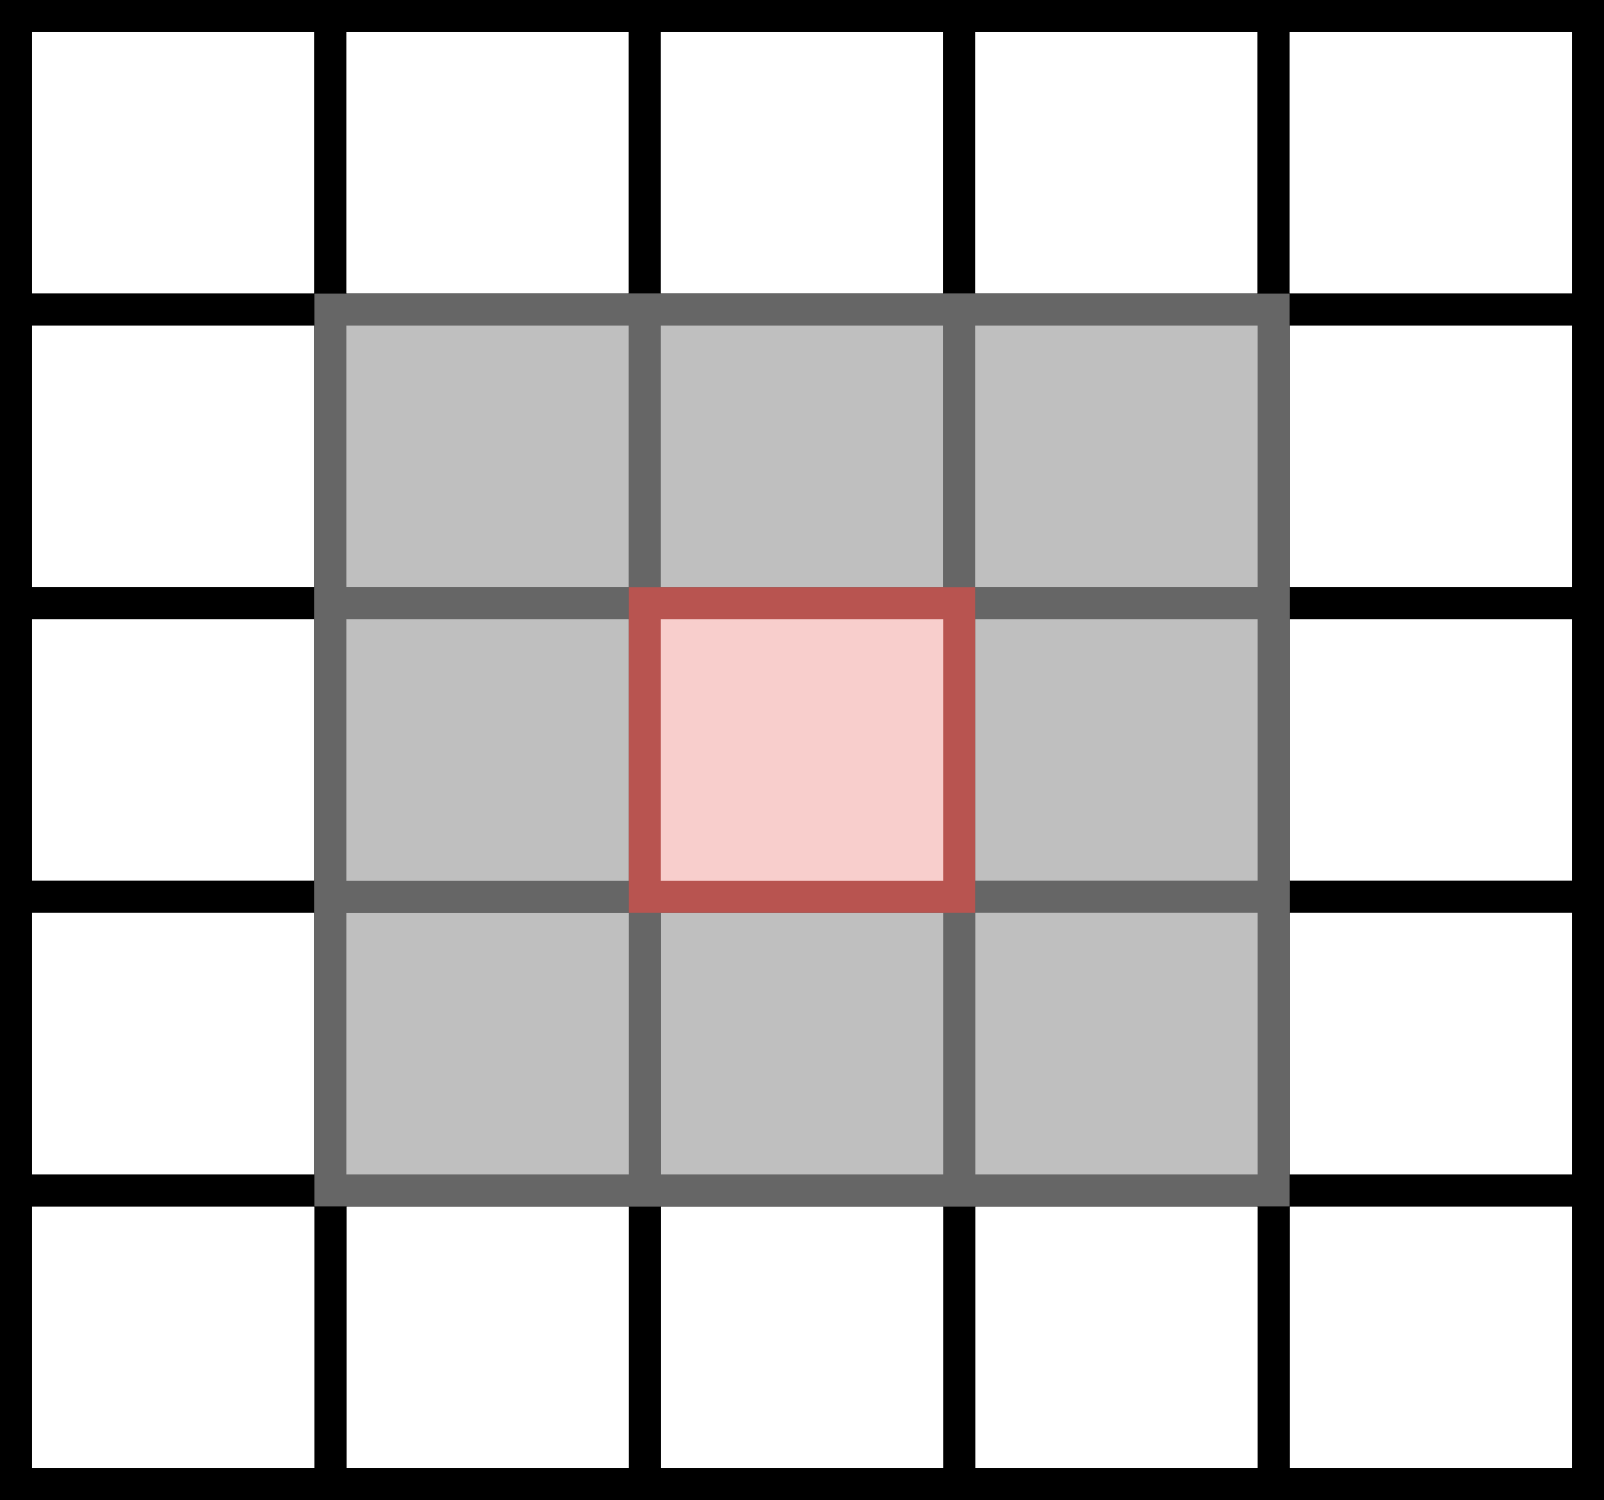
\includegraphics[height=4.5cm,width=4.5cm]{fig/moore.png}}}
\qquad
\subfloat[Von Neumann]{{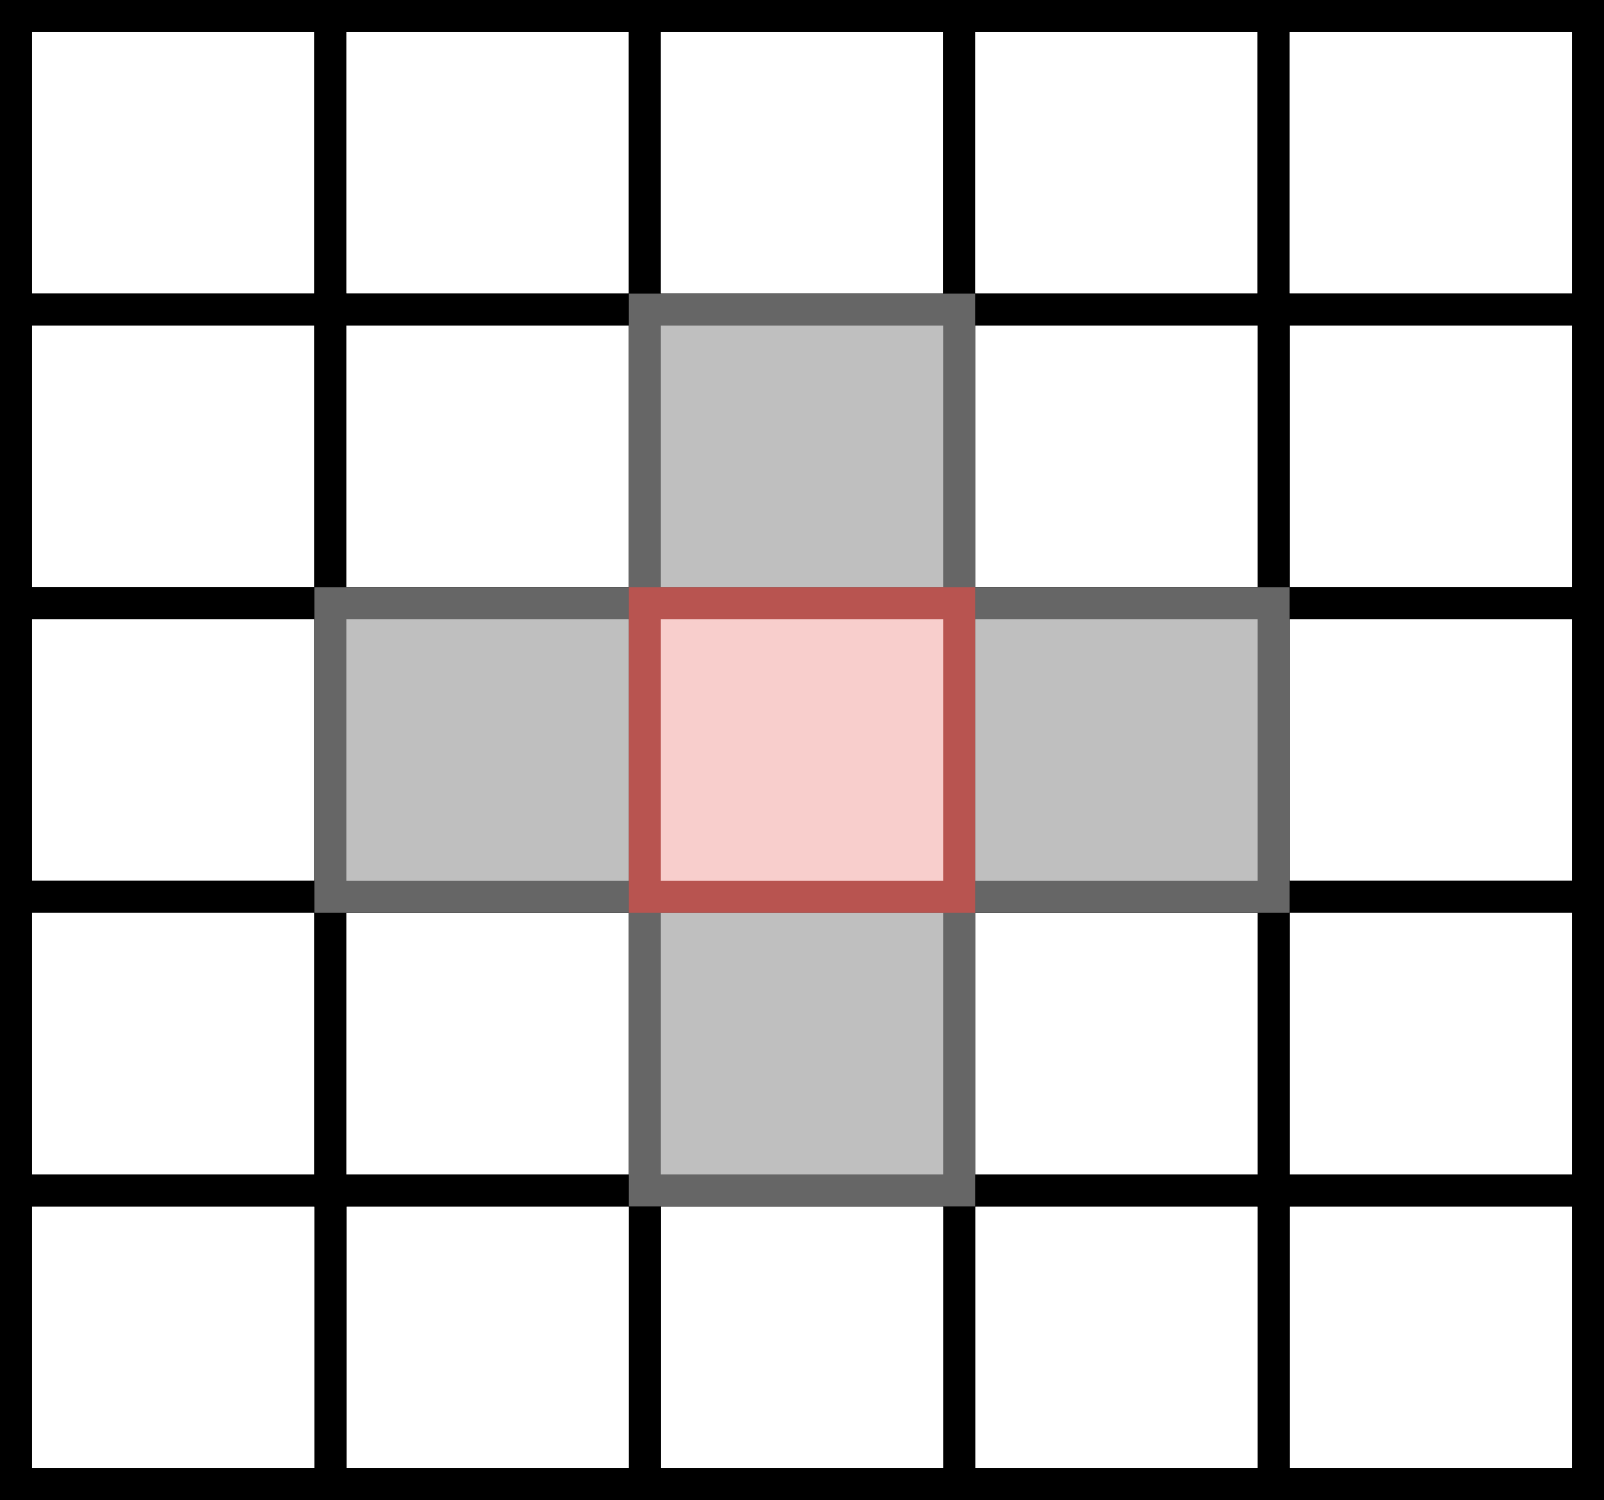
\includegraphics[height=4.5cm,width=4.5cm]{fig/vonneumann.png} }}
\qquad
\caption{Vizinhanças bidimensionais. Adaptado de ALEXANDER 2008\cite{alexanderschatten2008}}
\label{figure:neighbor}
\end{figure}

Através do espaço celular e do conceito de vizinhança as \texttt{Regras de transição} podem ser definidas, essas que através de um conjunto de condições, considerando o estado atual de cada célula e a de seus vizinhos, faz atualizações de estado em cada célula, sendo que, o estado atual sempre é definido pela análise dos estados anteriores (SHIFFMAN 2012\cite{Shiffman2012}).

O último componente é o \texttt{Tempo}, considerado como uma dimensão do autômato celular, é utilizado para determinar, em mudanças discretas (ALEXANDER 2008\cite{alexanderschatten2008}), a atualização dos estados através da aplicação das regras de transição, essas sendo feitas todas ao mesmo tempo, para todas as células (LIU 2008\cite{Liu2008}), de modo que, a atualização de um estado em um determinado tempo, não interfira. no resultado de outro no mesmo instante de tempo. \\

\section{Modelo de Propagação Epidêmica}
De acordo com White 2007\cite{White2007} e Sirakou 2000\cite{Sirakoulis2000}, modelos clássicos de propagação epidêmica podem não representam o problema como um todo, isso porque, ao aplicar equações diferenciais (Ordinárias ou Parciais), algumas características de epidemias são deixados de lado, a citar: $(i)$ O processo de contato individual; $(ii)$ comportamentos individuais; $(iii)$ aspectos espaciais da propagação; e $(iv)$ efeito dos padrões de mistura dos indivíduos.

Para contornar tais problemas, é proposto a utilização de ACs para a modelagem da propagação epidêmica (WHITE 2007\cite{White2007} e SIRAKOUS 2000\cite{Sirakoulis2000}). Melloti 2009\cite{Melotti2009} apresentam diversos exemplos de trabalhos que possuem bons resultados na modelagem de propagação epidêmica com AC são apresentados.

Neste contexto, o presente trabalho implementa e analisa um modelo determinístico, criado para a simulação geral de epidemias, proposto em White 2007\cite{White2007}. A explicação do modelo pode ser feita em duas partes, população e função de transição, cada uma dessas especificadas ao longo das subseções abaixo. \\

\subsection{População}
Como descrito por White 2007\cite{White2007}, para a representação da população dentro do AC é assumido que, o terreno onde a epidemia está ocorrendo representa o espaço celular bidimensional $MxN$, com células de geometria quadrada e áreas idênticas. Dentro de cada uma das células $(i,j)$ é tido que existe uma população de indivíduos $N_{ij}$, com distribuição não-homogênea, permitindo a existência de diferentes quantidades de indivíduos na população das diferentes células do espaço celular. Como o modelo apresentado neste trabalho é baseado em modelos Suscetíveis-Infectados-Recuperados (SIR), cada indivíduo dentro das populações das células podem ser dos tipos \texttt{suscetíveis}, \texttt{infectados} ou \texttt{recuperados}. Para este modelo, a população de cada célula é considerada como estado.

De forma geral, o que ocorre é, para cada tempo $t$ da simulação, em cada uma das células $(i,j)$ do espaço celular, poderão existir diferentes porcentagens de tipos de indivíduos diferentes, como apresentado na Figura \ref{figure:cellArticle}, sendo necessário considerar que a partição dos suscetíveis $S_{ij}^t \in [0, 1]$, a partição dos infectados $I_{ij}^t \in [0, 1]$ e a partição dos recuperados $R_{ij}^t \in [0, 1]$, juntas, devem respeitar a regra $S_{ij}^t + I_{ij}^t + R_{ij}^t = 1$ em cada célula.

Além disto, o modelo considera também que a epidemial não é letal e que também que não existem nascimentos durante a simulação, o que faz a população total ser constante, o que consequentemente faz com que todas as células sempre tenham a mesma quantidade de indivíduos em sua população.

\begin{figure}[ht]
 \begin{center}
  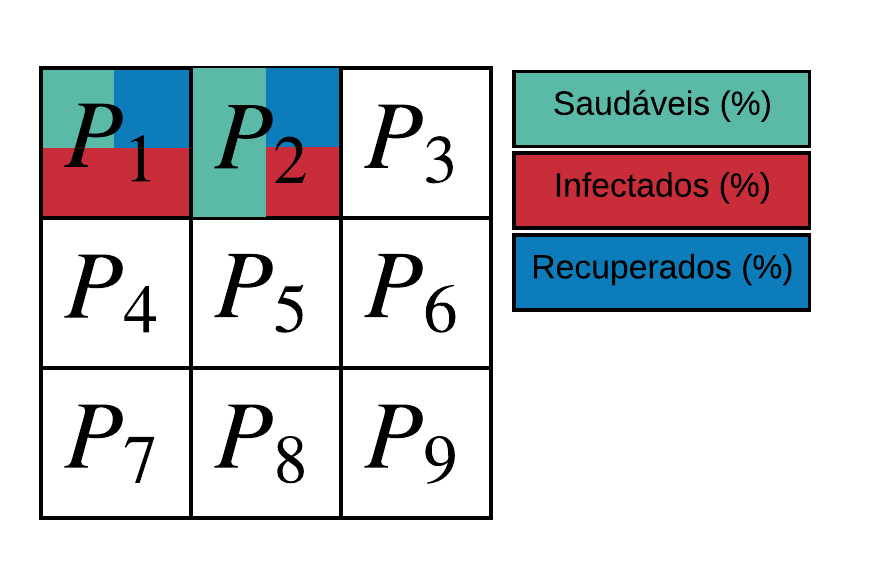
\includegraphics[width=0.7\linewidth]{fig/modelo_ca_artigo_v2.png}
 \end{center}
 \caption{Representação dos possíveis estados dos indivíduos dentro de uma células.}
\label{figure:cellArticle}
\end{figure}

Esta consideração faz também com que o processo de infecção seja modelado de forma diferente, no modelo estudado, só são infectados aqueles que estão suscetíveis, e após um tempo infectado é possível passar para o estado recuperado, sendo que, chegando neste estado, não há mais mudança de estado para tal indivíduo, é considerado que o mesmo desenvolveu imunidade contra o vírus propagado.

A maneira com que a infecção ocorre é descrita através da relação entre os indivíduos infectados da mesma célula ou com células vizinhas, o que garante que durante a simulação existirão meios de relacionamento intra e extra célula, sendo que, para extra células, meios de transportes são considerados. \\

\subsection{Função de transição}
As funções de transição, como já explicadas anteriormente, são as responsáveis em realizar a atualização dos estados das células com base no estado atual de cada célula e também o estado de seus vizinhos. O modelo estudado neste trabalho, utiliza as vizinhanças de \texttt{Moore} e \texttt{Von Neumann} (Figura \ref{figure:neighbor}) e considera três equações, uma para cada tipo de indivíduo da população vistos na seção anterior. As equações que definem o sistema são:

\begin{equation} 
I_{ij}^t=\left(1\:-\:\varepsilon \right)\cdot I_{ij}^{t\:-\:1}+v\:\cdot S_{ij}^{t\:-\:1}\cdot I_{ij}^{t\:-\:1}+S_{ij}^{t\:-\:1}\cdot \:\displaystyle \:\sum _{\left(\alpha ,\beta \right)\in V^{\ast }}^{ }\left(\frac{N_{i+\alpha ,\:j\:+\:\beta }}{N_{ij}}\cdot \mu _{\alpha \beta }^{\left(i,\:j\right)}\cdot I_{i+\alpha \:,\:j+\beta \:}^{t\:-\:1}\:\right)
\label{eq1}
\end{equation}

\begin{equation}
S_{ij}^t=S_{ij}^{t\:-\:1}-v\cdot S_{ij}^{t\:-\:1}\cdot I_{ij}^{t\:-\:1}-S_{ij}^{t\:-\:1}\cdot \:\displaystyle \:\sum _{\left(\alpha ,\beta \right)\in V^{\ast }}^{ }\left(\frac{N_{i+\alpha ,\:j\:+\:\beta }}{N_{ij}}\cdot \mu _{\alpha \beta }^{\left(i,\:j\right)}\cdot I_{i+\alpha \:,\:j+\beta \:}^{t\:-\:1}\:\right)
\label{eq2}
\end{equation}

\begin{equation} 
R_{ij}^t=R_{ij}^{t\:-\:1}+\varepsilon \cdot I_{ij}^{t\:-\:1}
\label{eq3}
\end{equation}

A variável $V^\star$ representa todos os vizinhos de uma célula e o parâmetro $\mu_{\alpha \beta}^{\left(i,\:j\right)}$ é definido como:

\begin{equation}
   \mu_{\alpha \beta}^{\left(i,\:j\right)} = c_{\alpha\beta}^{\left(i,\:j\right)} m_{\alpha \beta}^{\left(i,\:j\right)} v
\end{equation}

Onde $c_{\alpha \beta}^{\left(i,\:j\right)}$ e $ m_{\alpha \beta}^{\left(i,\:j\right)}$ representam o fator de conexão entre as células e o fator de movimento entre a célula e seus vizinhos $(i + \alpha, j + \beta)$, respectivamente. 

O fator $v \in [0, 1]$ representa a virulência da epidemia e $\varepsilon \in [0, 1]$, indica o fator de recuperação dos indivíduos infectados.

As equações \ref{eq1}, \ref{eq2} e \ref{eq3} apresentam um sistema conservativo, ou seja, caso haja um aumento na quantidade de um tipo de indivíduo, haverá a diminuição de outro tipo. Tal comportamento pode ser visto diretamente nas equações, por exemplo, para as equações \ref{eq1} e \ref{eq2} é possível perceber que existe uma relação onde, os indivíduos suscetíveis diminuirão caso o número de infectados aumente. A análise das equações pode ser feita através da interpretação de seus termos. 

Para a equação \ref{eq1}, na primeira soma, é tido que os infectados no instante de tempo $t$ serão representados pela porção de indivíduos do instante de tempo $t-1$ que não foram curados. O segundo termo mostra a porção dos indivíduos saudáveis que foram infectados pelo contato com infectados, isto considera o fator de virulência, este termo é proporcional na agressividade do vírus. A terceira soma apresenta os que foram infectados por contato com vizinhos infectados. Na equação \ref{eq2} tem-se comportamento análogo ao apresentado, porém considerando os suscetíveis. Já a equação \ref{eq3}, apresenta seu resultado como sendo o somatório da parcela dos infectados que são recuperados em cada instante de tempo $t$.

\subsection{Conexão e Movimento}
Para estes fatores é possível interpretar esses como sendo, respectivamente, a quantidade de serviços que o indivíduo tem disponível para sair de sua célula e ir para outra e o fator de movimento representa a necessidade do indivíduo de utilizar tais serviços. Durante a descrição do fator de escala, White 2007\cite{White2007} faz uma relação com meios de transporte como avião, ônibus e carro entre cada célula e determina um fator que represente cada um desses meios de transporte. Essa relação de fatores é apresentada na Tabela \ref{tab:movimentacao}. 

\begin{table}[ht]
 \caption{Discretização do transporte. Adaptado de WHITE 2007\cite{White2007}.}
 \centering
 \begin{tabular}{c|c|c|c|c}
  Conectividade & Fator & Avião & Ônibus & Carro \\
  \hline
  \multirow{4}{*}{$m_{\alpha \beta}^{\left(i,\:j\right)}$} & 1 & x & x & x \\
   & 0.6 & x & x & - \\
   & 0.3 & x & - & - \\
   & 0 & - & - & - \\
\end{tabular}
\label{tab:movimentacao}
\end{table}

% Não sei se precisa de tal explicação, a tabela está bem clara
% Onde a x determina sim o sistema possui o meio de transporte, além da Tabela \ref{tab:movimentacao}, tanto para a população quanto para a movimentação, ambos podem ser considerados como valores constantes para maior simplicidade.

\newpage
\subsection{Vacinação}
O AC analisado e implementado neste trabalho, considera também no comportamento dos indivíduos a adição de vacina contra o vírus da epidemia. As equações para este caso tem comportamento análogo ao já apresentado anteriormente, com a diferença de que, nessas que consideram a vacina há o fator $\omega \in [0, 1]$, que representa a quantidade de indivíduos vacinados em cada célula. Tais mudanças são apresentadas nas equações \ref{eq:vacineS} e \ref{eq:vacineR}, não havendo mudanças para o comportamento dos infectados.

\begin{equation} 
S_{ij}^t=S_{ij}^{t\:-\:1}-\omega \cdot S_{ij}^{t\:-\:1}-v\cdot \:S_{ij}^{t\:-\:1}\cdot \:I_{ij}^{t\:-\:1}-S_{ij}^{t\:-\:1}\cdot \:\displaystyle \:\sum _{\left(\alpha ,\beta \right)\in V^{\ast }}^{ }\left(\frac{N_{i+\alpha ,\:j\:+\:\beta }}{N_{ij}}\cdot \mu _{\alpha \beta }^{\left(i,\:j\right)}\cdot I_{i+\alpha \:,\:j+\beta \:}^{t\:-\:1}\:\right)
\label{eq:vacineS}
\end{equation}

\begin{equation} 
R_{ij}^t=R_{ij}^{t\:-\:1}+\varepsilon \:\cdot \:I_{ij}^{t\:-\:1}+\omega \cdot S_{ij}^{t\:-1}
\label{eq:vacineR}
\end{equation}

\section{Resultados}

Esta seção é dividida em duas partes, sendo que a primeira apresenta a implementação base do modelo com analises dos resultados seguindo os testes propostos em White 2007\cite{White2007}. Na segunda parte um exemplo de espacialização do modelo.\\

A utilização de diferentes plataformas para a implementação do modelo foi feita apenas para a comparação, sendo que, os passos para a implementação através do TerraME foram identificados como muito mais simples e claros, permitindo que toda a lógica do modelo fosse aplicada sem grandes preocupações com as maneiras de fazer, uma vez que a plataforma ofereceu todas as ferramentas necessárias para a mesma. As implementações\footnote{O código desenvolvido e animações criadas está disponível no GitHub (\href{https://github.com/M3nin0/epidemic-model}{https://bit.ly/2KfYnf7})} apresentadas foram feitas utilizando Python, para a espacialização do modelo, e a plataforma de modelagem TerraME (CARNEIRO 2013 \cite{CARNEIRO2013104}), que possibilita a rápida prototipação e desenvolvimento de modelos baseados em diferentes abordagens, utilizada para o entendimento do modelo implementado no trabalho.

%%---------------------------------------------
%% Parâmetros do modelo nos testes de espacialização do modelo 
%% ToDo: mover esta parte para dentro da seção da espacialização do 
% As condições do sistema foram:

% \begin{table}[ht]
%  \caption{Condições do sistema.}
%  \centering
%  \begin{tabular}{c|c|c}
%  Tempos & t & 200 \\
%  \hline
%  Virulência & v & 0.6 \\
%  Recuperação & $\varepsilon$ & 0.2 \\
%  Movimentação & m & 0.2
%  \end{tabular}
%  \label{tab:condicoes1}
% \end{table}

% Para as experiências realizadas em Python, o factor de recuperação, ou seja, a capacidade de recuperação dos indivíduos infectados, será igual a 0, a fim de facilitar a diferença entre as variáveis espaciais a comparar.
% Por conseguinte, para este cenário, o vírus infectará de forma imparável, apenas travado pela vacinação.

% \begin{table}[ht]
%  \caption{Condições do sistema.}
%  \centering
%  \begin{tabular}{c|c|c}
%  Tempos & t & 200 \\
%  \hline
%  Virulência & v & 0.6 \\
%  Recuperação & $\varepsilon$ & 0 \\
%  Movimentação & m & 0.2
%  \end{tabular}
%  \label{tab:condicoes2}
% \end{table}

%%---------------

\subsection{Simulações base}

Como forma de ilustrar o comportamento do modelo com diferentes conjuntos de parâmetros, esta seção faz diferentes testes variando os parâmetros de simulação do modelo. Para todos os testes é utilizado um espaço celular de 50x50, sendo que, o ponto inicial da epidemia em todos os casos ocorre a partir da célula $(25,25)$ e todas as células tem população $N_{ij}$ igual a 100.\\

O primeiro caso de testes assume o mesmo conjunto de parâmetros utilizados por White 2007\cite{White2007}, onde é aplicado na célula de início da epidemia que a população será dividida em 70\% de suscetíveis e 30\% de infectados, e que os valores dos parâmetros utilizados no modelo são, $v$ = 0.6, $\varepsilon$ = 0.4 e  $ m_{\alpha \beta}^{\left(i,\:j\right)}$ = 0.5. É considerado também que o fator de conexão $c_{\alpha \beta}^{\left(i,\:j\right)}$ é 1, para todas as células. 

\newpage
A Figura \ref{figure:exp1moore} apresenta os resultados da simulação utilizando a vizinhança de Moore e na Figura \ref{figure:exp1vonneumann} são apresentados os resultados da simulação com a vizinhança de Von Neumann. As cores das figuras representam a quantidade de infectados nas células, indo do branco ao vermelho, com tons de cinza como intermediários. Assim, o branco representa que não há infectados e o vermelho representa que toda a população da célula foi infectada. 

\begin{figure}[!ht]
\captionsetup[subfigure]{labelformat=empty}
\centering
\subfloat[\textit{t} = 1]{{\includegraphics[height=2.5cm,width=2.5cm, frame]{fig/experimentos_base/images_parametros_padrao_teste_modelo_moore/epidemicmodel_t1.png}}}
\qquad
\subfloat[\textit{t} = 5]{{\includegraphics[height=2.5cm,width=2.5cm, frame]{fig/experimentos_base/images_parametros_padrao_teste_modelo_moore/epidemicmodel_t5.png}}}
\qquad
\subfloat[\textit{t} = 15]{{
\includegraphics[height=2.5cm,width=2.5cm, frame]{fig/experimentos_base/images_parametros_padrao_teste_modelo_moore/epidemicmodel_t15.png}}}
\qquad
\subfloat[\textit{t} = 20]{{
\includegraphics[height=2.5cm,width=2.5cm, frame]{fig/experimentos_base/images_parametros_padrao_teste_modelo_moore/epidemicmodel_t20.png}}}
\qquad
\subfloat[\textit{t} = 25]{{
\includegraphics[height=2.5cm,width=2.5cm, frame]{fig/experimentos_base/images_parametros_padrao_teste_modelo_moore/epidemicmodel_t25.png}}}
\qquad
\subfloat[\textit{t} = 30]{{
\includegraphics[height=2.5cm,width=2.5cm, frame]{fig/experimentos_base/images_parametros_padrao_teste_modelo_moore/epidemicmodel_t30.png}}}
\qquad
\subfloat[\textit{t} = 35]{{
\includegraphics[height=2.5cm,width=2.5cm, frame]{fig/experimentos_base/images_parametros_padrao_teste_modelo_moore/epidemicmodel_t35.png}}}
\qquad
\subfloat[\textit{t} = 40]{{
\includegraphics[height=2.5cm,width=2.5cm, frame]{fig/experimentos_base/images_parametros_padrao_teste_modelo_moore/epidemicmodel_t40.png}}}
\caption{Simulação com população constante e vizinhança de Moore}
\label{figure:exp1moore}
\end{figure}

\begin{figure}[!ht]
\captionsetup[subfigure]{labelformat=empty}
\centering
\subfloat[\textit{t} = 1]{{\includegraphics[height=2.5cm,width=2.5cm, frame]{fig/experimentos_base/images_parametros_padrao_teste_modelo_vonneumann/epidemicmodel_t1.png}}}
\qquad
\subfloat[\textit{t} = 5]{{
\includegraphics[height=2.5cm,width=2.5cm, frame]{fig/experimentos_base/images_parametros_padrao_teste_modelo_vonneumann/epidemicmodel_t5.png}}}
\qquad
\subfloat[\textit{t} = 15]{{
\includegraphics[height=2.5cm,width=2.5cm, frame]{fig/experimentos_base/images_parametros_padrao_teste_modelo_vonneumann/epidemicmodel_t15.png}}}
\qquad
\subfloat[\textit{t} = 20]{{
\includegraphics[height=2.5cm,width=2.5cm, frame]{fig/experimentos_base/images_parametros_padrao_teste_modelo_vonneumann/epidemicmodel_t20.png}}}
\qquad
\subfloat[\textit{t} = 25]{{
\includegraphics[height=2.5cm,width=2.5cm, frame]{fig/experimentos_base/images_parametros_padrao_teste_modelo_vonneumann/epidemicmodel_t25.png}}}
\qquad
\subfloat[\textit{t} = 30]{{
\includegraphics[height=2.5cm,width=2.5cm, frame]{fig/experimentos_base/images_parametros_padrao_teste_modelo_vonneumann/epidemicmodel_t30.png}}}
\qquad
\subfloat[\textit{t} = 35]{{
\includegraphics[height=2.5cm,width=2.5cm, frame]{fig/experimentos_base/images_parametros_padrao_teste_modelo_vonneumann/epidemicmodel_t35.png}}}
\qquad
\subfloat[\textit{t} = 40]{{
\includegraphics[height=2.5cm,width=2.5cm, frame]{fig/experimentos_base/images_parametros_padrao_teste_modelo_vonneumann/epidemicmodel_t40.png}}}
\caption{Simulação com população constante e vizinhança de Von Neumann}
\label{figure:exp1vonneumann}
\end{figure}

Como é possível perceber nas figuras apresentadas, as simulações utilizando as vizinhanças de Moore apresentam estágios bem maiores de infecção do que as simulações feitas utilizando as vizinhanças de Von Neumann, o que pode ser explicado pela quantidade de vizinhos que cada célula tem contato de uma única vez. Ao ter mais contato com outras células, a chance de contaminação é grande. Como forma de visualizar a forma como cada uma das vizinhanças se comporta, a Figura \ref{figure:exp1graph}. 

\newpage
Partindo dos resultados desta simulação é importante entender a maneira como o fator de conexão entre as células afeta a epidemia modelada, o método de divisão do espaço celular, apresentado em (WHITE 2007\cite{White2007}) foi utilizando. Neste, o espaço celular é separado em quatro quadrantes, sendo que para cada quadrante um fator de conectividade (Tabela \ref{tab:movimentacao}), é utilizado. 

\begin{figure}[!ht]
\centering
\subfloat[Moore]{{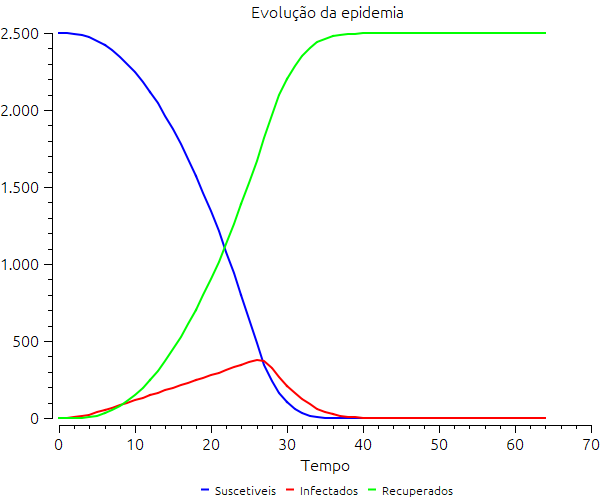
\includegraphics[height=5.5cm,width=5.5cm, frame]{fig/experimentos_base/images_parametros_padrao_teste_modelo_moore/epidemicmodel_finalchart.png}}}
\qquad
\subfloat[Von Neumann]{{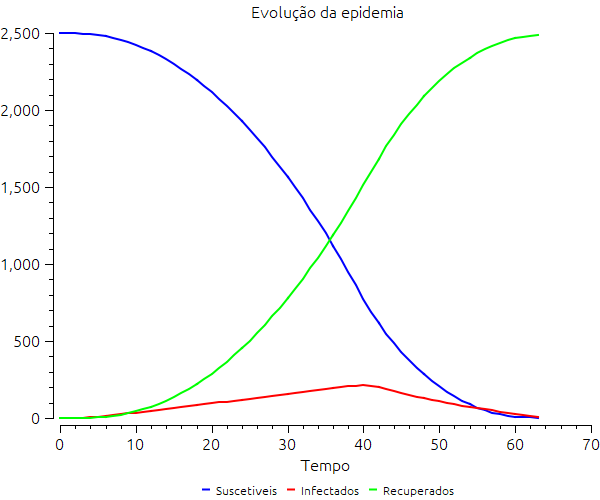
\includegraphics[height=5.5cm,width=5.5cm, frame]{fig/experimentos_base/images_parametros_padrao_teste_modelo_vonneumann/epidemicmodel_finalchart.png}}}
\caption{Simulação com diferentes formas de vizinhanças}
\label{figure:exp1graph}
\end{figure}

A distribuição das conectividades do espaço celular podem ser vistos na Figura \ref{figure:artificialCellSpace}, onde as tonalidades de cores representam o grau do fator de conexão, quanto mais escuro, maior o grau de conexão. Assim, as áreas $C_1$ e $C_2$ possuem os maiores fatores de conectividade, sendo respectivamente os valores 0.6 e 1. Já as áreas $C_3$ e $C_4$ possuem fatores de conectividade menor, sendo esses 0 e 0.3, respectivamente. 

\begin{figure}[!ht]
 \begin{center}
  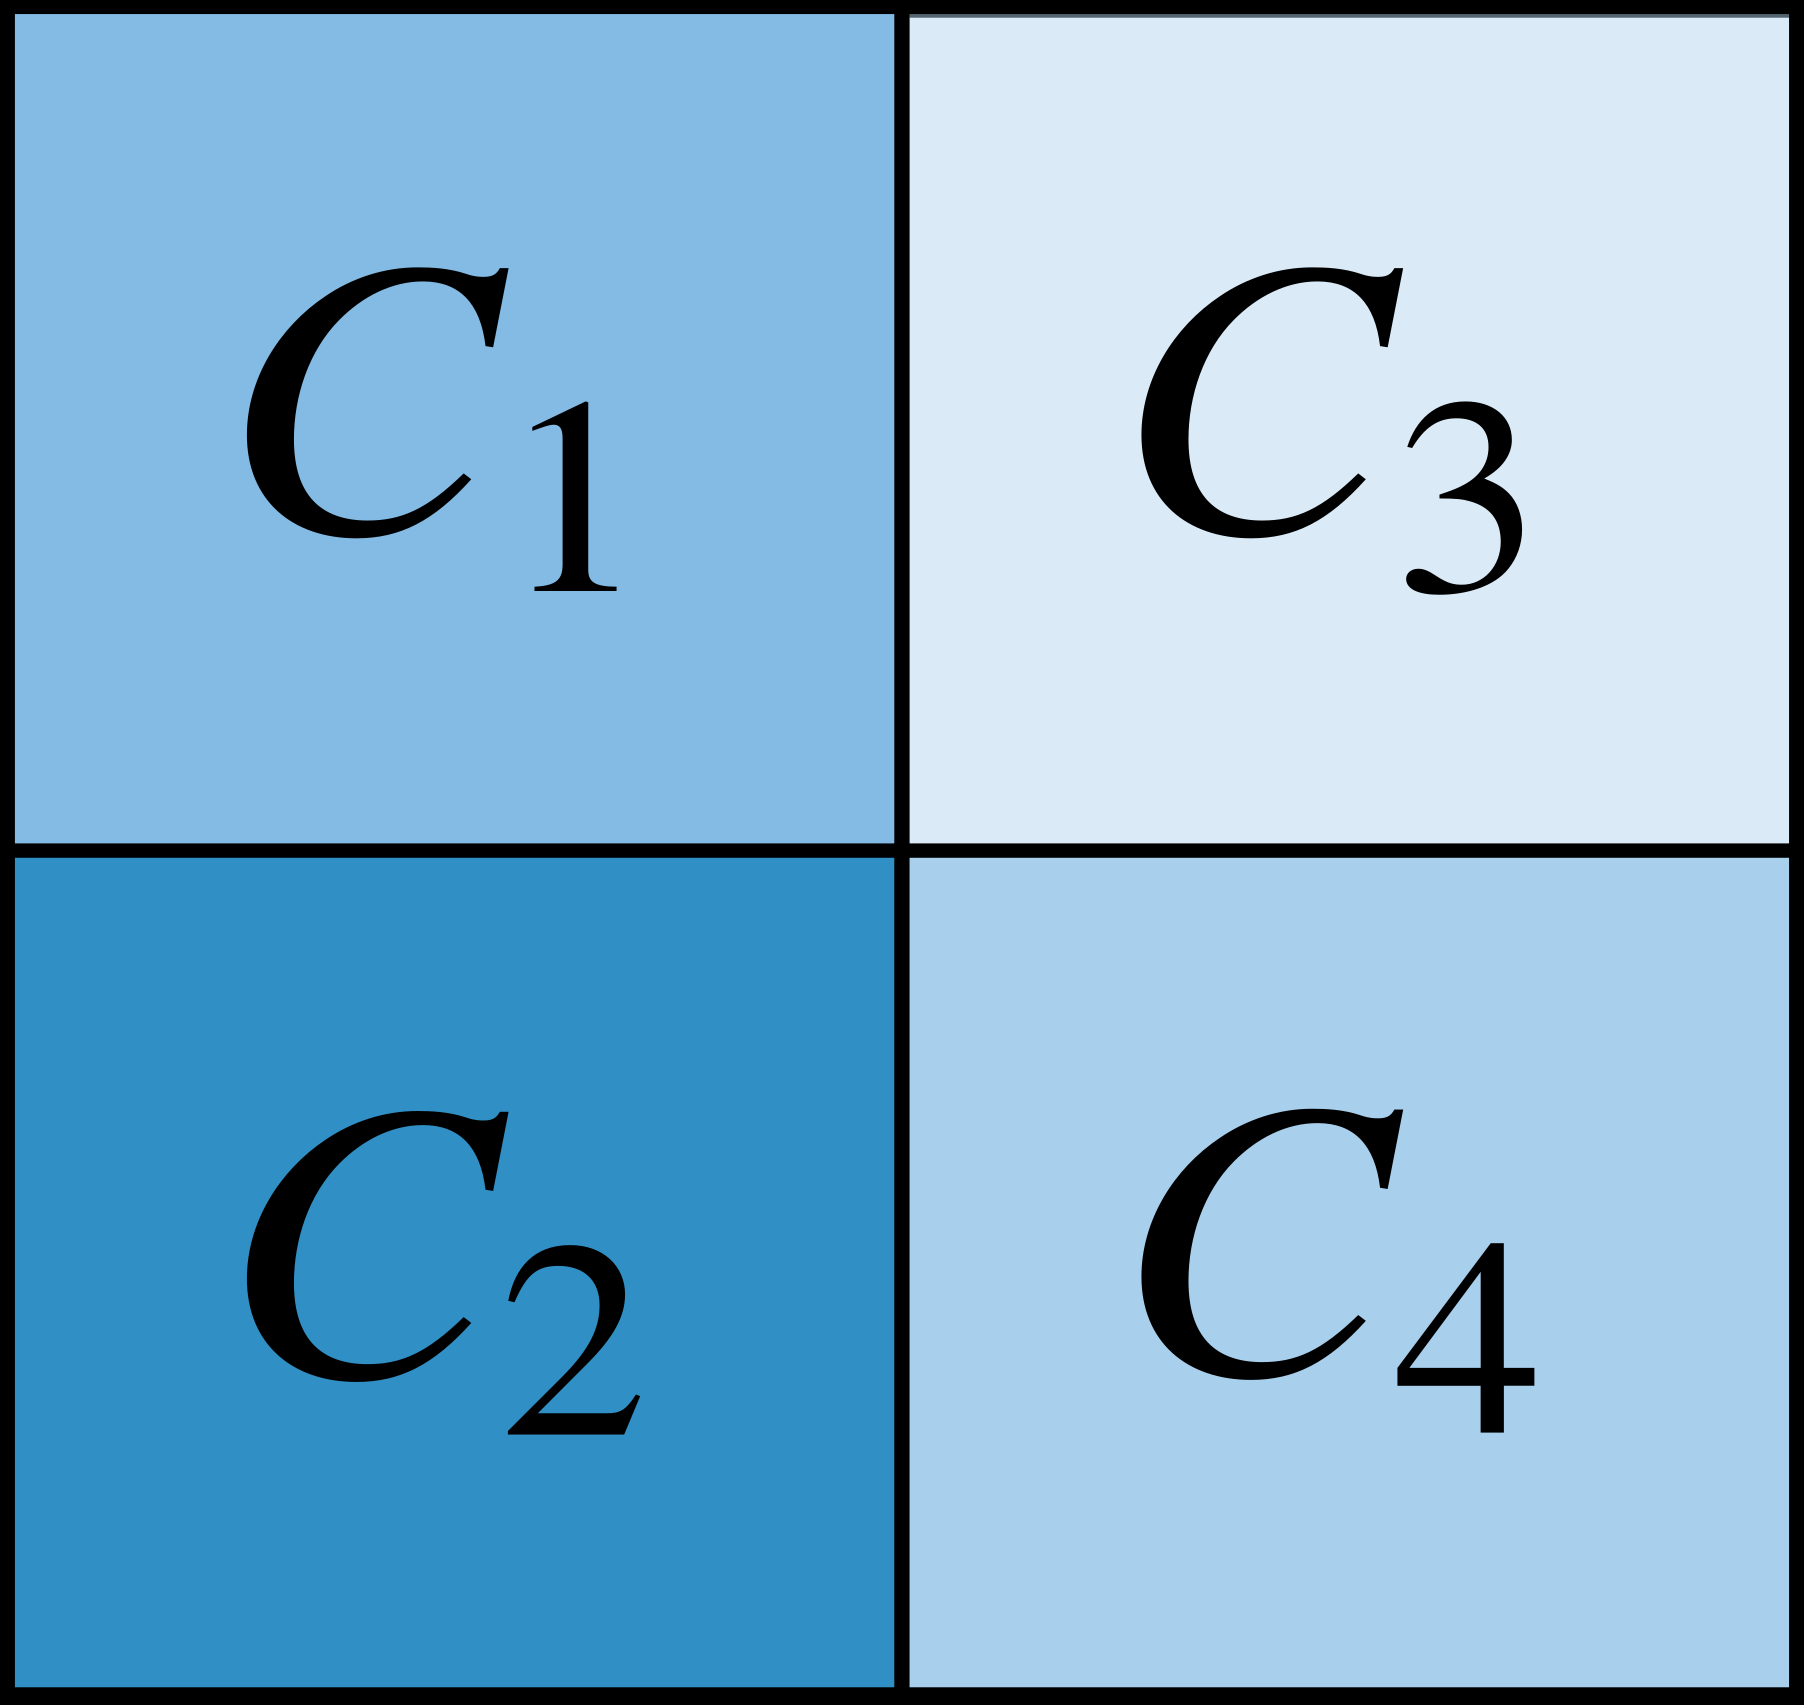
\includegraphics[width=0.35\linewidth]{fig/area_artificial.png}
 \end{center}
 \caption{Espaço celular com quadrantes diferentes de conectividade}
\label{figure:artificialCellSpace}
\end{figure}

Com isso, ao realizar as simulações, tanto para os testes de vizinhanças de Moore (Figura \ref{figure:exp2moore}) quanto de Von Neumann (Figura \ref{figure:exp2vonneumann}), é possível perceber que as áreas que representam $C_1$ e $C_2$, por dispor de maior conectividade, fizeram o vírus se espalhar mais rápido, enquanto que no quadrante $C_3$, por não possuir conexão com outras células, não teve nenhuma infecção e no $C_4$, em que a transmissão foi muito baixa. 

\newpage
É importante citar também que, o mesmo comportamento do número de infectados foi encontrado aqui, onde as simulações com Moore tiveram mais casos de células todas infectadas, quando comparadas com as simulações feitas com Von Neumann. \\

\begin{figure}[!ht]
\captionsetup[subfigure]{labelformat=empty}
\centering
\subfloat[\textit{t} = 1]{{\includegraphics[height=2.5cm,width=2.5cm, frame]{fig/experimentos_base/images_parametros_padrao_area_artificial_moore/epidemicmodel_t1.png}}}
\qquad
\subfloat[\textit{t} = 5]{{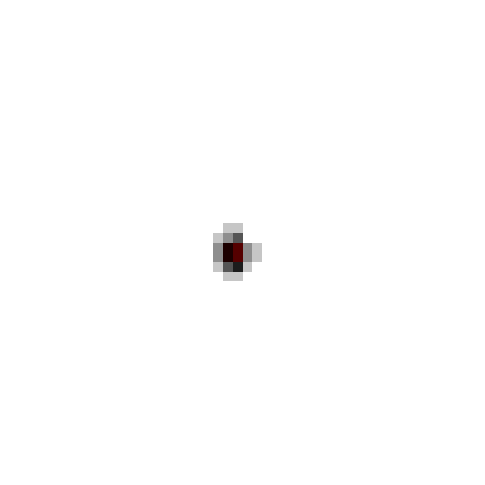
\includegraphics[height=2.5cm,width=2.5cm, frame]{fig/experimentos_base/images_parametros_padrao_area_artificial_moore/epidemicmodel_t5.png}}}
\qquad
\subfloat[\textit{t} = 10]{{
\includegraphics[height=2.5cm,width=2.5cm, frame]{fig/experimentos_base/images_parametros_padrao_area_artificial_moore/epidemicmodel_t10.png}}}
\qquad
\subfloat[\textit{t} = 15]{{
\includegraphics[height=2.5cm,width=2.5cm, frame]{fig/experimentos_base/images_parametros_padrao_area_artificial_moore/epidemicmodel_t15.png}}}
\qquad
\subfloat[\textit{t} = 25]{{
\includegraphics[height=2.5cm,width=2.5cm, frame]{fig/experimentos_base/images_parametros_padrao_area_artificial_moore/epidemicmodel_t25.png}}}
\qquad
\subfloat[\textit{t} = 35]{{
\includegraphics[height=2.5cm,width=2.5cm, frame]{fig/experimentos_base/images_parametros_padrao_area_artificial_moore/epidemicmodel_t35.png}}}
\qquad
\subfloat[\textit{t} = 50]{{
\includegraphics[height=2.5cm,width=2.5cm, frame]{fig/experimentos_base/images_parametros_padrao_area_artificial_moore/epidemicmodel_t50.png}}}
\qquad
\subfloat[\textit{t} = 60]{{
\includegraphics[height=2.5cm,width=2.5cm, frame]{fig/experimentos_base/images_parametros_padrao_area_artificial_moore/epidemicmodel_t65.png}}}
\caption{Simulação com população constante e vizinhança de Moore com conectividade por quadrante}
\label{figure:exp2moore}
\end{figure}

\begin{figure}[!ht]
\captionsetup[subfigure]{labelformat=empty}
\centering
\subfloat[\textit{t} = 1]{{\includegraphics[height=2.5cm,width=2.5cm, frame]{fig/experimentos_base/images_parametros_padrao_area_artificial_vonneumann/epidemicmodel_t1.png}}}
\qquad
\subfloat[\textit{t} = 5]{{
\includegraphics[height=2.5cm,width=2.5cm, frame]{fig/experimentos_base/images_parametros_padrao_area_artificial_vonneumann/epidemicmodel_t5.png}}}
\qquad
\subfloat[\textit{t} = 10]{{
\includegraphics[height=2.5cm,width=2.5cm, frame]{fig/experimentos_base/images_parametros_padrao_area_artificial_vonneumann/epidemicmodel_t10.png}}}
\qquad
\subfloat[\textit{t} = 15]{{
\includegraphics[height=2.5cm,width=2.5cm, frame]{fig/experimentos_base/images_parametros_padrao_area_artificial_vonneumann/epidemicmodel_t15.png}}}
\qquad
\subfloat[\textit{t} = 25]{{
\includegraphics[height=2.5cm,width=2.5cm, frame]{fig/experimentos_base/images_parametros_padrao_area_artificial_vonneumann/epidemicmodel_t25.png}}}
\qquad
\subfloat[\textit{t} = 35]{{
\includegraphics[height=2.5cm,width=2.5cm, frame]{fig/experimentos_base/images_parametros_padrao_area_artificial_vonneumann/epidemicmodel_t35.png}}}
\qquad
\subfloat[\textit{t} = 50]{{
\includegraphics[height=2.5cm,width=2.5cm, frame]{fig/experimentos_base/images_parametros_padrao_area_artificial_vonneumann/epidemicmodel_t50.png}}}
\qquad
\subfloat[\textit{t} = 60]{{
\includegraphics[height=2.5cm,width=2.5cm, frame]{fig/experimentos_base/images_parametros_padrao_area_artificial_vonneumann/epidemicmodel_t65.png}}}
\caption{Simulação com população constante e vizinhança de Von Neumann com conectividade por quadrante}
\label{figure:exp2vonneumann}
\end{figure}

Até este ponto, todas as simulações foram feitas com população constante, como já citado anteriormente, porém, o modelo analisado neste trabalho da margem para a variação da população, indicando que tal variação influência diretamente no efeito da epidemia que está sendo gerado, desta forma, seguindo o teste proposto por White 2007\cite{White2007}, a população em cada célula é definida por $e^j$, com isso, os quadrantes $C_2$ e $C_4$ possuem uma maior quantidade de população em cada célula. A Figura \ref{figure:exp3moore} apresenta os resultados da simulação, nesta é evidente que, mesmo com uma maior quantidade de população em cada célula, o fator de conectividade ainda continuou interferindo nos resultados. 

% Moore
\begin{figure}[!ht]
\captionsetup[subfigure]{labelformat=empty}
\centering
\subfloat[\textit{t} = 1]{{\includegraphics[height=2.5cm,width=2.5cm, frame]{fig/experimentos_base/images_parametros_padrao_area_artificial_moore_popnaohomogenea/epidemicmodel_t1.png}}}
\qquad
\subfloat[\textit{t} = 5]{{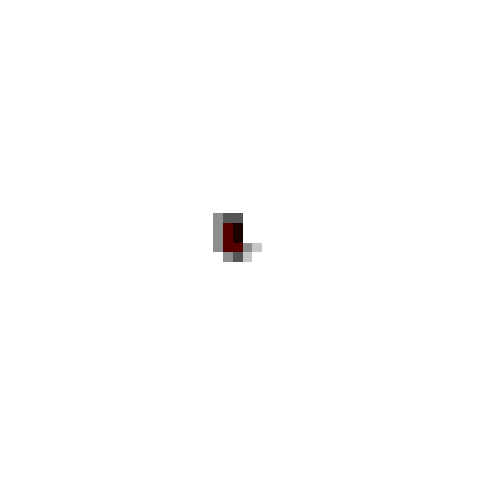
\includegraphics[height=2.5cm,width=2.5cm, frame]{fig/experimentos_base/images_parametros_padrao_area_artificial_moore_popnaohomogenea/epidemicmodel_t5.png}}}
\qquad
\subfloat[\textit{t} = 10]{{
\includegraphics[height=2.5cm,width=2.5cm, frame]{fig/experimentos_base/images_parametros_padrao_area_artificial_moore_popnaohomogenea/epidemicmodel_t10.png}}}
\qquad
\subfloat[\textit{t} = 15]{{
\includegraphics[height=2.5cm,width=2.5cm, frame]{fig/experimentos_base/images_parametros_padrao_area_artificial_moore_popnaohomogenea/epidemicmodel_t15.png}}}
\qquad
\subfloat[\textit{t} = 25]{{
\includegraphics[height=2.5cm,width=2.5cm, frame]{fig/experimentos_base/images_parametros_padrao_area_artificial_moore_popnaohomogenea/epidemicmodel_t25.png}}}
\qquad
\subfloat[\textit{t} = 35]{{
\includegraphics[height=2.5cm,width=2.5cm, frame]{fig/experimentos_base/images_parametros_padrao_area_artificial_moore_popnaohomogenea/epidemicmodel_t35.png}}}
\qquad
\subfloat[\textit{t} = 50]{{
\includegraphics[height=2.5cm,width=2.5cm, frame]{fig/experimentos_base/images_parametros_padrao_area_artificial_moore_popnaohomogenea/epidemicmodel_t50.png}}}
\qquad
\subfloat[\textit{t} = 60]{{
\includegraphics[height=2.5cm,width=2.5cm, frame]{fig/experimentos_base/images_parametros_padrao_area_artificial_moore_popnaohomogenea/epidemicmodel_t65.png}}}
\caption{Simulação com população variável ($e^j$) e vizinhança de Moore com conectividade por quadrante}
\label{figure:exp3moore}
\end{figure}

\subsubsection{Vacinação na população}

O modelo analisado neste trabalho, considera também a disponibilização de vacinas para o controle da epidemia que está sendo modelada. Desta forma, alguns testes considerando este parâmetro serão realizados, para estes, os mesmos parâmetros utilizados como padrão são empregados novamente nesta parte.\\

O primeiro teste realizado considera que o desenvolvimento e aplicação de uma vacina frente a uma epidemia não é imediato, desta forma, o fator de vacina começa somente a ser aplicado nas células somente após $t = 15$. A Figura \ref{figure:vac1moore} apresenta o resultado de uma simulação utilizando a vizinhança de Moore e um fator de vacinação $\omega = 0.2$, neste é possível perceber que, logo após a aplicação da vacina, a quantidade de infectados começa a diminuir de forma muito rápida. 

% vac1
\begin{figure}[!ht]
\captionsetup[subfigure]{labelformat=empty}
\centering
\subfloat[\textit{t} = 1]{{\includegraphics[height=2.5cm,width=2.5cm, frame]{fig/experimentos_base/images_parametros_padrao_vacina_0-2/epidemicmodel_t1.png}}}
\qquad
\subfloat[\textit{t} = 5]{{\includegraphics[height=2.5cm,width=2.5cm, frame]{fig/experimentos_base/images_parametros_padrao_vacina_0-2/epidemicmodel_t5.png}}}
\qquad
\subfloat[\textit{t} = 10]{{
\includegraphics[height=2.5cm,width=2.5cm, frame]{fig/experimentos_base/images_parametros_padrao_vacina_0-2/epidemicmodel_t10.png}}}
\qquad
\subfloat[\textit{t} = 15]{{\includegraphics[height=2.5cm,width=2.5cm, frame]{fig/experimentos_base/images_parametros_padrao_vacina_0-2/epidemicmodel_t15.png}}}
\qquad
\subfloat[\textit{t} = 18]{{\includegraphics[height=2.5cm,width=2.5cm, frame]{fig/experimentos_base/images_parametros_padrao_vacina_0-2/epidemicmodel_t18.png}}}
\qquad
\subfloat[\textit{t} = 20]{{\includegraphics[height=2.5cm,width=2.5cm, frame]{fig/experimentos_base/images_parametros_padrao_vacina_0-2/epidemicmodel_t20.png}}}
\qquad
\subfloat[\textit{t} = 21]{{\includegraphics[height=2.5cm,width=2.5cm, frame]{fig/experimentos_base/images_parametros_padrao_vacina_0-2/epidemicmodel_t21.png}}}
\qquad
\subfloat[\textit{t} = 23]{{\includegraphics[height=2.5cm,width=2.5cm, frame]{fig/experimentos_base/images_parametros_padrao_vacina_0-2/epidemicmodel_t23.png}}}
\caption{Simulação com população constante e vizinhança de Moore com vacinação igualmente distribuída}
\label{figure:vac1moore}
\end{figure}

\newpage
Como os parâmetros utilizados para este testes são os mesmos empregados anteriormente, é possível realizar um comparativo para entender a eficácia do fator de vacinação. Perceba que na Figura \ref{figure:exp1moore} a epidemia continua a se espalhar até o final do espaço celular, sendo que mesmo havendo recuperação dos indivíduos infectados, o vírus se manteria entre as população, mas, ao considerar a vacinação, como apresentado na Figura \ref{figure:vac1moore} a epidemia não foi apenas parada como a quantidade de infectados foi para zero, antes mesmo de atingir $t = 30$. É interessante notar que todo este comportamento ocorreu mesmo com um fator de vacinação $\omega$ pequeno. \\

Através do fator de vacinação é possível modelar muitos casos que se assemelham a comportamentos reais em casos de epidemia. Como forma de avaliação da junção de diferentes fatores, foi realizado um teste em que, a região de início da epidemia é no quadrante $C_1$, nesta existe um fator de vacina de $\omega = 0.1$ que está sendo aplicado para simular as tentativas da população de parar a epidemia, enquanto que nos demais quadrantes não existe este fator de vacinação. Além disto, o fato de conexão dentro deste quadrante é reduzido para $ m_{\alpha \beta}^{\left(i,\:j\right)}$ = 0.3, porém, nos demais quadrantes todas as operações continuam operando, ou seja, possuí valor igual a $ m_{\alpha \beta}^{\left(i,\:j\right)}$ = 1, o que pode ser utilizado para simular uma região tentando conter uma possível epidemia enquanto todas as demais continuam normalmente suas atividades. Os resultados desta simulação são apresentados na Figura \ref{figure:vac2moore}. 

% vac2
\begin{figure}[!ht]
\captionsetup[subfigure]{labelformat=empty}
\centering
\subfloat[\textit{t} = 1]{{\includegraphics[height=2.5cm,width=2.5cm, frame]{fig/experimentos_base/images_parametros_padrao_1quad_contaminado_com_vacina_0-10/epidemicmodel_t1.png}}}
\qquad
\subfloat[\textit{t} = 10]{{\includegraphics[height=2.5cm,width=2.5cm, frame]{fig/experimentos_base/images_parametros_padrao_1quad_contaminado_com_vacina_0-10/epidemicmodel_t10.png}}}
\qquad
\subfloat[\textit{t} = 15]{{\includegraphics[height=2.5cm,width=2.5cm, frame]{fig/experimentos_base/images_parametros_padrao_1quad_contaminado_com_vacina_0-10/epidemicmodel_t15.png}}}
\qquad
\subfloat[\textit{t} = 20]{{\includegraphics[height=2.5cm,width=2.5cm, frame]{fig/experimentos_base/images_parametros_padrao_1quad_contaminado_com_vacina_0-10/epidemicmodel_t20.png}}}
\qquad
\subfloat[\textit{t} = 24]{{\includegraphics[height=2.5cm,width=2.5cm, frame]{fig/experimentos_base/images_parametros_padrao_1quad_contaminado_com_vacina_0-10/epidemicmodel_t24.png}}}
\qquad
\subfloat[\textit{t} = 25]{{\includegraphics[height=2.5cm,width=2.5cm, frame]{fig/experimentos_base/images_parametros_padrao_1quad_contaminado_com_vacina_0-10/epidemicmodel_t25.png}}}
\qquad
\subfloat[\textit{t} = 30]{{\includegraphics[height=2.5cm,width=2.5cm, frame]{fig/experimentos_base/images_parametros_padrao_1quad_contaminado_com_vacina_0-10/epidemicmodel_t30.png}}}
\qquad
\subfloat[\textit{t} = 40]{{\includegraphics[height=2.5cm,width=2.5cm, frame]{fig/experimentos_base/images_parametros_padrao_1quad_contaminado_com_vacina_0-10/epidemicmodel_t40.png}}}
\caption{Simulação com população constante, vizinhança de Moore, movimentação constante e vacinação apenas no quadrante $C_1$}
\label{figure:vac2moore}
\end{figure}

Com a simulação da \ref{figure:vac2moore} é possível entender que no contexto modelado, mesmo o local onde a epidemia foi iniciado buscando conter a mesma, problemas de aumento da epidemia ocorrem caso as populações que possuem algum vínculo com esta não busquem prevenção, o que pode ser comparado a contextos reais em uma epidemia.

% von neumann
% Figuras retiradas para diminuir a quantidade de testes repetidos, mas se necessário, 
% já estão organizadas e prontas para serem utilizadas.
% \begin{figure}[!ht]
% \captionsetup[subfigure]{labelformat=empty}
% \centering
% \subfloat[\textit{t} = 1]{{\includegraphics[height=2.5cm,width=2.5cm, frame]{fig/experimentos_base/images_parametros_padrao_area_artificial_vonneumann_popnaohomogenea/epidemicmodel_t1.png}}}
% \qquad
% \subfloat[\textit{t} = 5]{{\includegraphics[height=2.5cm,width=2.5cm, frame]{fig/experimentos_base/images_parametros_padrao_area_artificial_vonneumann_popnaohomogenea/epidemicmodel_t5.png}}}
% \qquad
% \subfloat[\textit{t} = 10]{{\includegraphics[height=2.5cm,width=2.5cm, frame]{fig/experimentos_base/images_parametros_padrao_area_artificial_vonneumann_popnaohomogenea/epidemicmodel_t10.png}}}
% \qquad
% \subfloat[\textit{t} = 15]{{\includegraphics[height=2.5cm,width=2.5cm, frame]{fig/experimentos_base/images_parametros_padrao_area_artificial_vonneumann_popnaohomogenea/epidemicmodel_t15.png}}}
% \qquad
% \subfloat[\textit{t} = 25]{{\includegraphics[height=2.5cm,width=2.5cm, frame]{fig/experimentos_base/images_parametros_padrao_area_artificial_vonneumann_popnaohomogenea/epidemicmodel_t25.png}}}
% \qquad
% \subfloat[\textit{t} = 35]{{\includegraphics[height=2.5cm,width=2.5cm, frame]{fig/experimentos_base/images_parametros_padrao_area_artificial_vonneumann_popnaohomogenea/epidemicmodel_t35.png}}}
% \qquad
% \subfloat[\textit{t} = 50]{{\includegraphics[height=2.5cm,width=2.5cm, frame]{fig/experimentos_base/images_parametros_padrao_area_artificial_vonneumann_popnaohomogenea/epidemicmodel_t50.png}}}
% \qquad
% \subfloat[\textit{t} = 60]{{\includegraphics[height=2.5cm,width=2.5cm, frame]{fig/experimentos_base/images_parametros_padrao_area_artificial_vonneumann_popnaohomogenea/epidemicmodel_t65.png}}}
% \caption{}
% \label{figure:exp1vonneumann}
% \end{figure}

%------------------------------------------------------------------

% \subsubsection{Experimento 3}
% Testes com diferentes parâmetros, mostrando que as limitações impostas pelo artigo são válidas.

\newpage
\subsection{Espacialização do modelo}

Como forma de estender a aplicação do modelo, foi realizado um processo de espacialização do mesmo, onde todas as regras definidas e formas de vizinhanças foram aplicadas sobre um espaço geográfico. A área de aplicação do modelo representa o território brasileiro, dividido em células para gerar o espaço celular, estes que possuem condições espaciais para população, conectividade e fator de vacinação, tomando como base para esses parâmetros as seguintes informações:

\begin{itemize}
    \item População: A população de cada estado;
    \item Conectividade: O numero de aeroportos por estado;
    \item Vacinação: Proporcional ao desenvolvimento econômico.
\end{itemize}

A Figura \ref{figure:CI} apresenta a forma e intensidade que cada uma dessas variáveis teve em seus respectivos estados.

Com o objetivo de obter a variável mais sensível em relação ao velocidade de expansão do vírus foram feitos os experimentos da Tabela \ref{tab:exp}.

\begin{table}[ht]
 \caption{Experimentos realizados no modelo espacializado}
 \centering
 \begin{tabular}{c|c|c|c|c}
  Experimento & Vizinhança & População & Conectividade & Vacinação \\
  \hline
  \multirow{2}{*}{1} & Moore & \multirow{2}{*}{Homogênea} & \multirow{2}{*}{Homogênea} & \multirow{2}{*}{Não} \\
   & Neumman &  &  &  \\
  \hline
  \multirow{2}{*}{2} & \multirow{2}{*}{Moore} & Homogênea & \multirow{2}{*}{Homogênea} & \multirow{2}{*}{Não} \\
  &  & Heterogênea &  &  \\
  \hline
  \multirow{2}{*}{3} & \multirow{2}{*}{Moore} & \multirow{2}{*}{Homogênea} & Homogênea & \multirow{2}{*}{Não} \\
  &  &  & Heterogênea &  \\
  \hline
  \multirow{2}{*}{4} & \multirow{2}{*}{Moore} & \multirow{2}{*}{Homogênea} & \multirow{2}{*}{Homogênea} & Sim \\
  &  &  &  & Não \\
\end{tabular}
\label{tab:exp}
\end{table}

\begin{figure}[!ht]
 \begin{center}
  \includegraphics[width=1\linewidth]{fig/variaveis_espaciais.png}
 \end{center}
 \caption{Condições espaciais heterogêneas.}
\label{figure:CI}
\end{figure}

\newpage
% Para cada experimento, das quatro variáveis uma e considerada heterogênea, isto apresenta variação espacial por enquanto as outras três são homogêneas e assim verificar a variação na velocidade da epidemia.\\

Para a condição espacial inicial da epidemia, ou seja, o local onde o vírus modelado é iniciado foi definido como o estado de São Paulo, como apresentado na Figura \ref{figure:CI_virus}. Esta condição será utilizada em todos os experimentos listados na Tabela \ref{figure:CI_virus} \\

\begin{figure}[!ht]
 \begin{center}
  \includegraphics[width=0.45\linewidth]{fig/ponto_inicial_virus.png}
 \end{center}
 \caption{Ponto inicial do vírus.}
\label{figure:CI_virus}
\end{figure}

Os parâmetros iniciais considerados em todos os experimentos são apresentados na Tabela \ref{tab:condicoes2}, onde o fator de recuperação, ou seja, a capacidade de recuperação dos indivíduos infectados, será igual a 0, a fim de facilitar a diferença entre as variáveis espaciais consideradas (tipo de vizinhança, população, conectividade e vacinação). Por conseguinte, neste cenário, o vírus infectará de forma a ser parado apenas com vacinas.

\begin{table}[ht]
 \caption{Condições do sistema.}
 \centering
 \begin{tabular}{c|c|c}
 Tempos & t & 200 \\
 \hline
 Virulência & v & 0.6 \\
 Recuperação & $\varepsilon$ & 0 \\
 Movimentação & m & 0.2
 \end{tabular}
 \label{tab:condicoes2}
\end{table}


\newpage
\subsubsection{Experimento 1}
\label{sub:exp1}

Este experimento apresenta a diferença entre os tipos de vizinhança, onde, para o primeiro gráfico foi utilizada a vizinhança de Moore e para o segundo a vizinhança Neumann (Figura \ref{figure:neighbor}), enquanto a população e a conectividade foram consideradas constantes e a vacinação igual a zero.

\begin{figure}[!ht]
 \begin{center}
  \includegraphics[width=1\linewidth]{fig/Vecino.png}
 \end{center}
 \caption{Evolução do vírus para os dois tipos de vizinhança.}
\label{figure:vizinho}
\end{figure}

\newpage
\subsubsection{Experimento 2}
\label{sub:exp2}

Para este experimento, foi utilizada a vizinhança de Moore porque a expansão é maior, enquanto a população foi considerada variável, seguindo  os valores da Figura \ref{figure:CI}, a conectividade permanece constante e a vacinação é zero.

\begin{figure}[!ht]
 \begin{center}
  \includegraphics[width=1\linewidth]{fig/Poblacion.png}
 \end{center}
 \caption{Evolução do vírus para variações de População.}
\label{figure:populacao}
\end{figure}

\newpage
\subsubsection{Experimento 3}
\label{sub:exp3}
O que se segue mostra a influência da conectividade na propagação do vírus, utilizando a vizinhança de Moore, uma população constante e sem a presença da vacinação.

\begin{figure}[!ht]
 \begin{center}
  \includegraphics[width=1\linewidth]{fig/Conectividad.png}
 \end{center}
 \caption{Evolução do vírus para variações de conectividade.}
\label{figure:conec}
\end{figure}

\newpage
\subsubsection{Experimento 4}
\label{sub:exp4}
Agora, considerando a existência de um programa de vacinação heterogêneo, isto significa que a variável vacinação diferirá entre alguns estados, foi utilizada a vizinhança de Moore, população e conectividade heterogênea, estes com o objectivo de uma maior velocidade de contágio para verificar a eficácia da vacina.

\begin{figure}[!ht]
 \begin{center}
  \includegraphics[width=1\linewidth]{fig/Vacuna.png}
 \end{center}
 \caption{Evolução do vírus com presença de vacinação.}
\label{figure:vacun}
\end{figure}

\newpage

\section{Conclusões}

Ao utilizar um modelo em que os indivíduos não apresentam capacidade de recuperação, como pode ser visto nos experimentos das secções \ref{sub:exp1}, \ref{sub:exp2} e \ref{sub:exp3}, as áreas atingidas pelo vírus apresentam uma infecção do $100\%$, portanto, estes casos não existem indivíduos recuperados, tanto naturalmente como pela ausência de vacinação. 

No caso da variação de vizinhança (Figura \ref{figure:exp1moore} e \ref{figure:vizinho}), a vizinhança de Moore ao considerar um número maior de vizinhos (Figura \ref{figure:neighbor}) permite uma dispersão da infecção muito mais rápida em relação a vizinhança de Neumann. Para os experimentos 2 e 3 (Figura \ref{figure:conec} e \ref{figure:populacao}), campos não homogêneos de população e conectividade foram utilizadas, respectivamente, em comparação com as condições constantes destas (ou seja, população e conectividade iguais a $1$ para todos os estados).
Em ambos casos, maior população e maior conectividade fizeram a epidemia atinger um número maior de pessoas suscetíveis. No entanto, a Figura \ref{figure:conec} - \texttt{Abs Diff} mostra que variações na conectividade geram maior velocidade de propagação em comparação com a variações da população, por exemplo, no experimento 2 (seção \ref{sub:exp2}) onde o número de pessoas infectadas chega a 1500 por volta do tempo 170, enquanto que no experimento 3 (Seção \ref{sub:exp3}) o mesmo número foi alcançado por volta do tempo 120, sendo que o experimento 3 apresenta uma maior velocidade de infecção. 

A Figura \ref{figure:vac1moore} mostra este cenário com vacinação homogeneamente distribuída, neste é possível perceber a eficiência da vacinação frente a epidemia modelada, já que logo após a aplicação da vacina o numero de infectados começa a diminuir. A Figura \ref{figure:vac2moore} apresenta apenas no quadrante $C_1$ com fator de vacinação, nesta Figura pode-se observar a diferença entre a evolução do vírus dentro do quadrante com vacinação e fora dele, onde o número de pessoas infectadas é muito maior. Para o experimento 4 (Seção \ref{sub:exp4}) foi adicionado um fator de vacinação (Tabela \ref{tab:exp}), que para este caso é a única maneira de impedir o avanço do vírus. 

No mapa de vacinação apresentado na Figura \ref{figure:CI}, o Sul, Sudeste e Nordeste de Brasil apresentam programas de vacinação e o Norte e Centro-Oeste não. Ao considerar tal mapa, ao visualizar a Figura \ref{figure:vacun} pode-se observar que os estados com maior fator de vacinação são os que apresentaram o menor numero de infectados. Por exemplo, devido ao programa de vacinação presente em São Paulo ter fator igual a 0.2, o avanço do vírus é muito menor do que em um cenário sem presença de vacina, o que também ocorre em estados com fator de vacinação igual ou próximo, como Minas Gerais, Santa Catarina, Rio Grande do Sul e Rio de Janeiro. Porém, ao considerar estados como Paraná, que possuem um fator de vacinação igual a 0.1, o número de infectados é muito maior, podendo neste caso, ser até mesmo considerado o maior na região sul do Brasil. Para os estados que não têm vacinação, no tempo 200 o vírus volta quase à sua capacidade máxima de infecção como pode ser visto nas regiões centro-oeste e norte do Brasil.

Com isto, é possível afirmar que o modelo implementado e analisado neste trabalho, mesmo não realizando considerações complexas do espalhamento de uma epidemia, consegue realizar a modelagem de cenários próximos aos de epidemias reais.

\newpage
\bibliographystyle{acm}
\bibliography{bibfile}

\end{document}

